\documentclass{article}
\usepackage{tikz}
\usetikzlibrary{automata,positioning}

\begin{document}

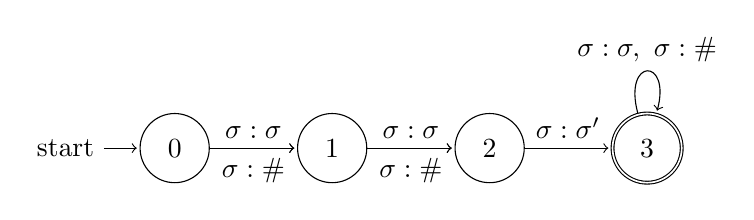
\begin{tikzpicture}[shorten >=1pt,node distance=2cm,on grid,auto]
    \node[state,initial] (q_0) {$0$};
    \node[state] (q_1) [right=of q_0] {$1$};
    \node[state] (q_2) [right=of q_1] {$2$};
    \node[state,accepting] (q_3) [right=of q_2] {$3$};

    \path[->]
        (q_0) edge node {$\sigma:\sigma$} (q_1)
              edge node [below] {$\sigma:\#$} (q_1)
        (q_1) edge node {$\sigma:\sigma$} (q_2)
              edge node [below] {$\sigma:\#$} (q_2)
        (q_2) edge node {$\sigma:\sigma'$} (q_3)
        (q_3) edge [loop above] node {$\sigma:\sigma,\ \sigma:\#$} ();
\end{tikzpicture}

\end{document}